% \documentclass{standalone}
% \usepackage{currfile,hyperxmp}

% \input{../tikz_header.tex}

% \begin{document}



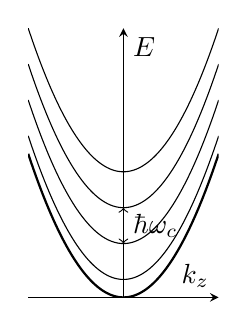
\begin{tikzpicture}
%\useasboundingbox (-1.3,-1.2) rectangle (10.2,4.7);
%\draw (-1,-1) rectangle (4,4);

    \begin{axis}[ xlabel={$k_z$}, ylabel={$E$}, 
         width=40mm, height=50mm, 
        %xmode=log, ymode=log,
         %xmin = -2,xmax=2,
         % ymin = 0, ymax=7.5,
         axis x line=middle,
         axis y line=middle,
         xtick = \empty, xticklabel = \empty,
         ytick = \empty, yticklabel = \empty,
         % xmax= 2e5, unbounded coords=jump, ymin=0, ymax = 4
        % label style={font=\tiny},
        % tick label style={font=\tiny}  
    ]


    \addplot[no marks, thick, color=black, domain = -2:2,samples=100,smooth] {x^2};
    \addplot[no marks, thin, color=black, domain = -2:2,samples=100,smooth] {x^2 + 0.5};
    \addplot[no marks, thin, color=black, domain = -2:2,samples=100,smooth] {x^2 + 1.5};
    \addplot[no marks, thin, color=black, domain = -2:2,samples=100,smooth] {x^2 + 2.5};
    \addplot[no marks, thin, color=black, domain = -2:2,samples=100,smooth] {x^2 + 3.5};

	 \draw [<->] (axis cs:0,1.5) -- node[right] {$\hbar \omega_c$} (axis cs: 0,2.5) ;

 

    \end{axis}
\end{tikzpicture}

%\end{document}